% Diese Datei ist Teil des Buchs "Schreibe Dein Programm!"
% Das Buch ist lizensiert unter der Creative-Commons-Lizenz
% "Namensnennung - Weitergabe unter gleichen Bedingungen 4.0 International (CC BY-SA 4.0)"
% https://creativecommons.org/licenses/by-sa/4.0/deed.de

\chapter{Programmieren mit Akkumulatoren}
\label{cha:accu}

Manche Berechnungen funktionieren am einfachsten, wenn sie ein
Zwischenergebnis mitführen und aktualisieren.  Die bisherigen
Konstruktionsanleitungen für Funktionen, die Listen oder natürliche
Zahlen verarbeiten, können das aber nicht.  Wir brauchen dafür eine
neue Programmiertechnik, das das Programmieren mit
\textit{Akkumulatoren}, und entsprechend angepasste
Konstruktionsanleitungen.  Beides gibt es in diesem Kapitel.

\section{Zwischenergebnisse mitführen}
\label{sec:intermediate-results}

Wir fangen mit einer scheinbar einfachen Funktion an: Gefragt ist eine
Funktion, die eine Liste invertiert, also die Reihenfolge ihrer
Elemente umdreht:\index{invert@\texttt{invert}}\label{sec:invert}
%
\begin{lstlisting}
; Liste umdrehen
(: invert ((list-of %a) -> (list-of %a)))

(check-expect (invert empty) empty)
(check-expect (invert (list 1 2 3 4)) (list 4 3 2 1))
\end{lstlisting}
%
Gerüst und Schablone sehen wie folgt aus:
%
\begin{lstlisting}
(define invert
  (lambda (list)
    (cond
      ((empty? list) ...)
      ((cons? list)
      ... (invert (rest list)) ...
      ... (first list) ...))))
\end{lstlisting}
%
Um den Rumpf zu vervollständigen, können wir uns an dem zweiten
Testfall orientieren~-- da ist \lstinline{list} die Liste mit den
Elementen 1 2 3 4.  Entsprechend ist \lstinline{(first list)} die
Zahl 1, \lstinline{(rest list)} die Liste mit den Elementen 2 3 4, das
heiß der rekursive Aufruf liefert die Liste mit den Elementen 4 3 2.
Um das gewünschte Ergebnis mit den Elementen 4 3 2 1 zu bekommen,
müssen wir deshalb \lstinline{(first list)} hinten an das Ergebnis des
rekursiven Aufrufs anhängen.

Um ein Element \emph{hinten} an eine Liste zu hängen, haben wir bisher
noch keine fertige Funktion~-- die müssen wir erst noch schreiben.
Wir könnten die Arbeit jetzt unterbrechen, um das zu tun.  Wir machen
erstmal nur eine Notiz, dass wir das später machen~-- in Form einer
Kurzbeschreibung und einer Signatur:0
%
\begin{lstlisting}
; Element an Liste anhängen
(: append-element ((list-of %a) %a -> (list-of %a)))
\end{lstlisting}
%
Wenn wir diese Funktion voraussetzen, können wir \lstinline{invert}
recht einfach fertigschreiben:
%
\begin{lstlisting}
(define invert
  (lambda (list)
    (cond
      ((empty? list) empty)
      ((cons? list)
       (append-element (invert (rest list))
                       (first list))))))
\end{lstlisting}
%
Die Funktion \lstinline{append-element} ist ganz ähnlich der Funktion
\lstinline{concatenate} aus Abschnitt~\ref{sec:more-lists}.  Zunächst
Testfälle:
%
\begin{lstlisting}
(check-expect (append-element (list 1 2 3) 4) (list 1 2 3 4))
(check-expect (append-element empty 4) (list 4))
\end{lstlisting}
%
Gerüst und Schablone:
%
\begin{lstlisting}
(define append-element
  (lambda (list element)
    (cond
      ((empty? list) ...)
      ((cons? list)
       ... (first list) ...
       ... (append-element (rest list) element) ...))))
\end{lstlisting}
%
Im \lstinline{cons}-Fall können wir auch hier die Lösung anhand eines
Beispiels finden: Im Testfall hat \lstinline{list} die Elemente 1 2 3,
der rekursive Aufruf liefert also 2 3 4.  Wir müssen
\lstinline{(first list)}, also die 1, nur noch vorne dranhängen, mit
\lstinline{cons}. Im \lstinline{empty}-Fall hängen wir
\lstinline{element} hinten an eine leere Liste~-- wir brauchen deshalb
eine einelementige Liste mit \lstinline{element} drin, das könnten wir
mit der eingebauten \lstinline{list} machen:
%
\begin{lstlisting}
(define append-element
  (lambda (list element)
    (cond
      ((empty? list) (list element))
      ((cons? list)
       (cons (first list)
             (append-element (rest list) element))))))
\end{lstlisting}
%
Hier wollten wir gern "<Fertig!"> wir sonst auch schreiben, aber die
Funktion funktioniert nicht: DrRacket beschwert sich, dass nach der
öffnenden Klammer von \lstinline{(list element)} keine Funktion steht
sondern \lstinline{#<empty-list>}.  Wups!  Das liegt daran, dass wir
den Namen \lstinline{list} auch für den Parameter gleichen Namens
verwendet haben.  Und nach den Regeln der lexikalischen Bindung aus
Abschnitt~\ref{sec:lexikalische-bindung} auf
Seite~\pageref{sec:lexikalische-bindung} überdeckt der Parameter die
eingebaute Funktion.

Wir können das Problem auf zwei Arten lösen~-- wir benennen den
Parameter um oder wir konstruieren die einelementige Liste "<von
Hand">.  Wir haben uns für letzteres entschieden:
%
\begin{lstlisting}
(define append-element
  (lambda (list element)
    (cond
      ((empty? list) (cons element empty))
      ((cons? list)
       (cons (first list)
             (append-element (rest list) element))))))
\end{lstlisting}

Doch zurück zu \lstinline{invert}.  Obwohl die zu erledigende Aufgabe
einfach erscheint, dauert schon das Invertieren von Listen der Länge
1000 eine ganze Weile.  Du kannst das zum Beispiel ausprobieren, indem
Du die Funktion \lstinline{copies} aus Abschnitt~\ref{func:copies} auf
Seite~\pageref{func:copies} verwendest und
%
\begin{lstlisting}
(invert (copies 1000 42))
\end{lstlisting}
%
Das dauert 2020 auf dem kaum ein Jahr alten Computer von Michael
Sperber immerhin ein
paar Sekunden: Das wäre vielleicht in den 70er Jahren noch akzeptabel
gewesen.  Tatsächlich ist es so, dass zum Beispiel
das Invertieren einer Liste der Länge 400 \emph{mehr} als doppelt so
lang wie das Invertieren einer Liste der Länge 200 benötigt.  Das
liegt daran, dass \lstinline{invert} bei jedem rekursiven Aufruf
\lstinline{append-element} aufruft, und \lstinline{append-element} selbst
macht soviele rekursive Aufrufe wie die Liste lang ist. Das sind für
eine Liste der Länge 20 für den ersten Aufruf von
\lstinline{append-element} 19 Aufrufe, für den zweiten 18 Aufrufe
undsoweiter.

Das sind also $19+18+17+\ldots+1$ rekursive Aufrufe.  Vielleicht
erinnerst Du Dich~-- das ist ein Beispiel für die Gaußsche
Summenformel, die wir in Abschnitt~\ref{sec:gausssche-summenformel}
auf Seite~\pageref{sec:gausssche-summenformel} bewiesen haben:
%
\[\forall n\in\mathbb{N}: \sum_{i=0}^n i =
  \frac{n\times (n+1)}{2}\]
%
\begin{figure}[tb]
  \centering
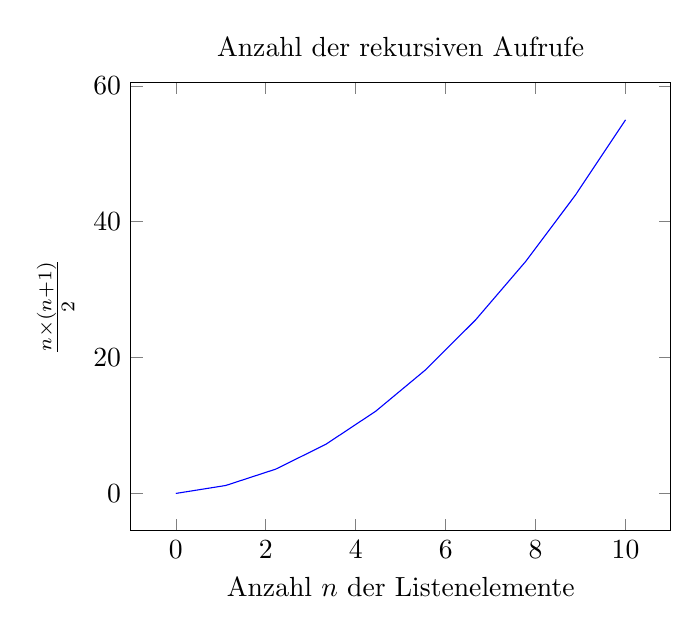
\begin{tikzpicture}
  \begin{axis}[
    title={Anzahl der rekursiven Aufrufe},
    xlabel={Anzahl $n$ der Listenelemente},
    ylabel={$\frac{n\times (n+1)}{2}$}
    ]
    \addplot [
    blue,
    domain=0:10,
    samples=10,
    ]
    {x*(x+1)/2};
  \end{axis}
\end{tikzpicture}
  \caption{Funktionaufrufe bei \lstinline{invert}}
  \label{fig:invert-calls}
\end{figure}

\noindent Wenn Du diese Formel für immer größer werdende $n$ ausrechnest, wird
die Zahl schwindelerregend schnell größer, wie
Abbildung~\ref{fig:invert-calls} zeigt.  Woran liegt das?

Wenn Du die rechte Seite ausmultiplizierst, steht da:
\[ \frac{n\times (n+1)}{2} = \frac{n^2 + n}{2} \]
%
In der Formel bestimmt das $n^2$ das schnelle Wachstum, auch
\textit{quadratisch} genannt.\index{quadratisches Wachstum}.  

Tatsächlich gibt es eine bessere Methode, eine Liste umzudrehen: Die
obige \lstinline{invert}"=Funktion konstruiert die Ergebnisliste, indem
stets Elemente \emph{hinten} angehängt werden.  Das entspricht 
nicht der "<natürlichen"> Konstruktion von Listen mit
\lstinline{cons}, das ein Element \emph{vorn} anhängt.  
Das Ergebnis ließe sich aber durch Anhängen vorn ganz einfach
konstruieren, und zwar, indem in folgender Reihenfolge
Zwischenergebnisse\index{Zwischenergebnis} berechnet werden, wie in folgendem Beispiel für den
Testfall \lstinline{(invert (list 1 2 3 4))}:
%
\begin{lstlisting}
#<empty-list>
#<list 1>
#<list 2 1>
#<list 3 2 1>
#<list 4 3 2 1>
\end{lstlisting}
%
Jedes Zwischenergebnis entsteht aus dem vorhergehenden, indem ein
Element vorn an die Liste darüber angehängt wird.  Dies geschieht in
der Reihenfolge, in der die Elemente in der ursprünglichen Liste
auftreten: scheinbar einfach.  Allerdings erlaubt die normale
Konstruktionsanleitung für Listen nicht, dieses Zwischenergebnis
mitzuführen: Das Ergebnis des rekursiven Aufrufs
\lstinline{(invert (rest lis))} ist unabhängig vom Wert von
\lstinline{(first lis)}.  Damit aber
ist es der Funktion aus der normalen Konstruktionsanleitung unmöglich,
die obige Folge von Zwischenergebnissen nachzuvollziehen, da von einem
Zwischenergebnis zum nächsten gerade \lstinline{(first lis)} vorn
angehängt wird.  Wir müssen also etwas anders an das Problem herangehen.

Um das Zwischenergebnis mitzuführen, 
benutzen wir einen separaten Parameter, einen sogenannten
\textit{Akkumulator\index{Akkumulator}}.  Dieser sammelt die
invertierte Liste der bisher schon "<gesehenen"> Elemente auf.  Hier
ist die Signatur der neuen Funktion \lstinline{invert-helper}:
%
\begin{lstlisting}
; Hilfsfunktion zum Umdrehen einer Liste
(: invert-helper ((list-of %a) (list-of %a) -> (list-of %a)))
\end{lstlisting}
%
Der folgende Testfall soll illustrieren, wie die Funktion arbeitet:
\begin{lstlisting}
(check-expect (invert-helper (list 4 5 6) (list 3 2 1))
              (list 6 5 4 3 2 1))
\end{lstlisting}
%
Die zweite Liste~-- der Akkumulator~-- enthält die "<bereits
invertierten"> Elemente.  Die erste Liste ist noch nicht verarbeitet;
die Elemente werden nacheinander an den Akkumulator vorn drangehängt.
Für die Definition der Funktion setzen wir erst einmal die bereits
bekannte Schablone ein für Funktionen, die eine Liste akzeptieren:
%
\begin{lstlisting}
(define invert-helper
  (lambda (list inverted)
    (cond
      ((empty? list) ...)
      ((cons? list)
       ... (first list) ...
       ... (invert-helper (rest list) ...) ...))))
\end{lstlisting}
%
Ziemlich viele Lücken noch!  Füllen wir erstmal die einfachste, im
\lstinline{empty}-Fall: Dann nämlich hat die Funktion schon "<alle
Elemente gesehen"> und diese in den Akkumulator \lstinline{inverted}
"<hineinakkumuliert">~-- der enthält dann die invertierte
Eingabeliste:
%
\begin{lstlisting}
(define invert-helper
  (lambda (list inverted)
    (cond
      ((empty? list) inverted)
      ((cons? list)
       ... (first list) ...
       ... (invert-helper (rest list) ...) ...))))
\end{lstlisting}
%
Im \lstinline{cons}-Fall müssen wir insbesondere das Argument zum zweiten
Parameter von \lstinline{invert-helper} ergänzen: Wir sind natürlich
versucht, da einfach \lstinline{inverted} hinzuschreiben wie bei
vielen anderen rekursiven Funktionen vorher.  Aber wir müssen doch die
Elemente von \lstinline{list} da noch "<hineinakkumulieren"> und aus
dem vorigen Zwischenergebnis das nächste machen.  Für das
"<Hineinakkumulieren"> nehmen wir das erste Elemente und hängen es
vorn an, so wie wir es in der Beispielrechnung auch gemacht haben:
%
\begin{lstlisting}
(define invert-helper
  (lambda (list inverted)
    (cond
      ((empty? list) inverted)
      ((cons? list)
       ...
       (invert-helper (rest list)
                      (cons (first list) inverted))
       ...))))
\end{lstlisting}
%
Was müssen wir noch dazuschreiben?  Die Funktion arbeitet schon die
Eingabeliste ab und akkumuliert ihre Elemente in \lstinline{inverted}
hinein: Sie ist bereits fertig, wir müssen nur die Ellipsen wegmachen:
%
\begin{lstlisting}
(define invert-helper
  (lambda (list inverted)
    (cond
      ((empty? list) inverted)
      ((cons? list)
       (invert-helper (rest list)
                      (cons (first list) inverted))))))
\end{lstlisting}
%
Die Funktion kann schon was, ist aber natürlich nicht identisch zur
ursprünglichen \lstinline{invert}-Funktion, die ja nur eine Eingabe
hat.  Um "<einfach nur eine Liste umzudrehen">, können wir
\lstinline{invert-helper} mit einem leeren Akkumulator aufrufen, wie
in diesem Testfall:
%
\begin{lstlisting}
(check-expect (invert-helper (list 1 2 3) empty)
              (list 3 2 1))
\end{lstlisting}
%
\begin{aufgabeinline}
  Definiere \lstinline{invert} um, so dass es
  \lstinline{invert-helper} benutzt!
\end{aufgabeinline}
%
Die neue Version von \lstinline{invert} funktioniert nicht nur
korrekt, sondern auch schnell: Sie benutzt keine Hilfsfunktion und
macht soviele rekursive Aufrufe wie die Eingabeliste Elemente hat, ihre
Laufzeit wächst also \textit{linear}.\index{lineares Wachstum}
Dass das so ist, kannst Du sehen, wenn Du die Auswertung eines Aufrufs
von \lstinline{invert} nachvollziehst:
%
\begin{alltt}\small
(invert \underline{(list 1 2 3 4)})
\(\ldots\evalsto\) (\underline{invert-helper} #<list 1 2 3 4> empty)
\(\ldots\evalsto\) (cond ((empty? #<list 1 2 3 4>) ...) ((cons? #<list 1 2 3 4>) ...))
\(\ldots\evalsto\) (invert-helper (rest #<list 1 2 3 4>) (cons (first #<list 1 2 3 4>) empty))
\(\ldots\evalsto\) (invert-helper #<list 2 3 4> (cons 1 empty))
\(\ldots\evalsto\) (invert-helper #<list 2 3 4> #<list 1>)
\(\ldots\evalsto\) (cond ((empty? #<list 2 3 4>) ...) ((cons? #<list 2 3 4>) ...))
\(\ldots\evalsto\) (invert-helper (rest #<list 2 3 4>) (cons (first #<list 2 3 4>) #<list 1>))
\(\ldots\evalsto\) (invert-helper #<list 3 4> (cons 2 #<list 1>))
\(\ldots\evalsto\) (invert-helper #<list 3 4> #<list 2 1>)
\(\ldots\evalsto\) (cond ((empty? #<list 3 4>) ...) ((cons? #<list 3 4>) ...))
\(\ldots\evalsto\) (invert-helper (rest #<list 3 4>) (cons (first #<list 3 4>) #<list 2 1>))
\(\ldots\evalsto\) (invert-helper #<list 4> (cons 3 #<list 2 1>))
\(\ldots\evalsto\) (invert-helper #<list 4> #<list 3 2 1>)
\(\ldots\evalsto\) (cond ((empty? #<list 4>) ...) ((cons? #<list 4>) ...))
\(\ldots\evalsto\) (invert-helper (rest #<list 4>) (cons (first #<list 4>) empty))
\(\ldots\evalsto\) (invert-helper #<empty-list> (cons 4 #<list 3 2 1>))
\(\ldots\evalsto\) (invert-helper #<empty-list> #<list 4 3 2 1>)
\(\ldots\evalsto\) (cond ((empty? #<empty-list>) #<list 4 3 2 1>) ((cons? #<empty-list>) ...))
\(\evalsto\) #<list 4 3 2 1>
\end{alltt}
%
Die höherere Effizienz hat allerdings auch ihren Preis.  Du merkst
vielleicht, dass auffällig viele der Erläuterungen hier in
Anführungszeichen stehen.  Das liegt daran, dass wir gar nicht so
einfach erklären können, wie wir die neue Funktion konstruiert haben.

Übrigens: Da die Funktion \lstinline{invert} generell nützlich ist,
ist sie unter dem Namen
\lstinline{reverse}\index{reverse@\texttt{reverse}} fest eingebaut.

\section{Schablonen für Funktionen mit Akkumulator}

Auch für Funktionen mit Akkumulator wollen wir eine
Konstruktionsanleitung entwickeln.  Vorher wollen wir aber noch einmal
anhand eines weiteren Beispiels Revue passieren lassen, wie der
Konstruktionsprozess bei solchen Funktionen eigentlich genau aussieht.

Wir nehmen uns eine Funktion vor, die wir eigentlich schon kennen,
nämlich aus Abschnitt~\ref{sec:list-sum} auf Seite
\pageref{sec:list-sum}:
%
\begin{lstlisting}
; Summe der Elemente einer Liste von Zahlen berechnen
(: list-sum ((list-of number) -> number))
\end{lstlisting}
%
Wir nehmen uns allerdings diesmal vor, mit Akkumulator zu arbeiten.
Dazu müssen wir uns erst einmal überlegen, was für Information der
Akkumulator eigentlich akkumulieren soll.  Das sollte ein
\textit{Zwischenergebnis}\index{Zwischenergebnis} sein, das ist oft
eine vorläufige Version des gewünschten Endergebnisses.  Da es 
hier das Endergebnis die Summe aller Listenelemente ist, nehmen wir
als Zwischenergebnis die Summer aller Listenelemente, die unsere
Funktion schon "<gesehen"> hat.  Wir nennen deshalb den
Akkumulator \lstinline{sum} und schreiben folgende Schablone:
%
\begin{lstlisting}
(define list-sum-helper
  (lambda (list sum)
    (cond
      ((empty? list) ... sum ...)
      ((cons? list)
       (list-sum-helper (rest list) (... (first list) ... sum ...))))))
\end{lstlisting}
%
Warum sieht sie gerade so aus beziehungsweise: Was ist der Unterschied
zur ganz normalen Schablone für Listen als Eingabe aus
Konstruktionsanleitung~\ref{ka:listen-eingabe-schablone} auf
Seite~\pageref{ka:listen-eingabe-schablone}?   Hier ist sie zur
Erinnerung noch einmal:
%
\begin{lstlisting}
(define |\(f\)|
  (lambda (|\ldots| |\(\mathit{list}\)| |\ldots|)
    (cond
      ((empty? |\(\mathit{list}\)|) |\ldots|)
      ((cons? |\(\mathit{list}\)|)
       |\ldots|
       (first |\(\mathit{list}\)|)
       (|\(f\)| (first |\(\mathit{list}\)|))
       |\ldots|
       ))))
\end{lstlisting}
%
Im \lstinline{empty}-Zweig steht der Akkumulator \lstinline{sum}, in
der Schablone aus
Konstruktionsanleitung~\ref{ka:listen-eingabe-schablone} gar nichts
steht: Hier ist die Liste am Ende und es ist Zeit, das Endergebnis
auszurechnen: das soll im \lstinline{empty}-Zweig herauskommen.   Weil
der Akkumulator ein Zwischenergebnis ist, muss er eine Rolle bei der
Berechnung des Endergebnisses spielen.  (Wir werden noch sehen, dass
das Endergebnis am Ende fast immer das letzte Zwischenergebnis
\emph{ist} beziehungsweise eine leichte Variation davon.)

Im \lstinline{cons}-Fall steht ein rekursiver Aufruf mit
\lstinline{(rest list)} als Listen-Argument~-- wie in
Konstruktionsanleitung~\ref{ka:listen-eingabe-schablone} auch.
Außerdem steht dort eine Hilfestellung für die Berechnung des
Akkumulator"=Arguments, also des nächsten Zwischenergebnisses.  Da
sollte das letzte Zwischenergebnis~-- hier \lstinline{sum}~-- und das
nächste Listenelement \lstinline{(first list)} eingehen. Darum stehen
sie in der Schablone.  Dieser Teil der Schablone ist also nur eine
Erweiterung der ursprünglichen Schablone.

Außerdem fällt Dir vielleicht auf, dass um den rekursiven Aufruf herum
keine Ellipsen \lstinline{...}: Du solltest da nichts drumherum
schreiben.  Das liegt daran, dass der letzte rekursive Aufruf von
\lstinline{list-sum-helper} am Ende der Liste das Ergebnis
produziert~-- das muss die Funktion einfach unverändert zurückliefern,
und darum steht da nichts drumherum.

Um die Funktion zu vervollständigen, müssen wir noch klarer als bisher
formulieren, was genau der Akkumulator \lstinline{sum} repräsentiert.
Oben haben wir etwas salopp geschrieben, dass es sich um die Summe
aller Listenelemente handelt, welche die Funktion schon "<gesehen">
hat.  Die sind aber für \lstinline{list-sum-helper} gar nicht mehr
sichtbar.  Wir können sie sichtbar machen, indem wir die Funktion
\lstinline{list-sum} einbeziehen, die \lstinline{list-sum-helper}
aufruft.  Hier ist ihre Schablone dafür:
%
\begin{lstlisting}
(define list-sum
  (lambda (list0)
    (list-sum-helper list0 ...)))
\end{lstlisting}
%
Wir haben bewusst den Namen \lstinline{list0} gewählt, damit wir ihn
nicht mit dem \lstinline{list} aus \lstinline{list-sum-helper}
durcheinanderbringen.  (Anders als noch bei \lstinline{reverse}~-- wir
versuchen es besser zu machen.)

\begin{figure}[tb]
  \centering
  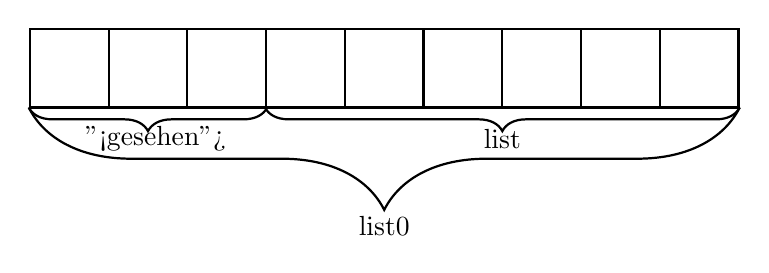
\begin{tikzpicture}
    \node (cell1) at (0,0) [draw,thick,minimum width=1cm,minimum height=1cm] {};
    \node (cell2) at (1,0) [draw,thick,minimum width=1cm,minimum height=1cm] {};
    \node (cell3) at (2,0) [draw,thick,minimum width=1cm,minimum height=1cm] {};
    \node (cell4) at (3,0) [draw,thick,minimum width=1cm,minimum height=1cm] {};
    \node (cell5) at (4,0) [draw,thick,minimum width=1cm,minimum height=1cm] {};
    \node (cell6) at (5,0) [draw,thick,minimum width=1cm,minimum height=1cm] {};
    \node (cell7) at (6,0) [draw,thick,minimum width=1cm,minimum height=1cm] {};
    \node (cell8) at (7,0) [draw,thick,minimum width=1cm,minimum height=1cm] {};
    \node (cell9) at (8,0) [draw,thick,minimum width=1cm,minimum height=1cm] {};
    \draw [
    thick,
    decoration={
        brace,
        amplitude=0.3cm,
        mirror,
        raise=0.5cm
    },
    decorate
    ] (cell4.west) -- (cell9.east) 
    node [midway,yshift=-0.9cm] {\lstinline{list}};
    \draw [
    thick,
    decoration={
        brace,
        amplitude=1.3cm,
        mirror,
        raise=0.5cm
    },
    decorate
    ] (cell1.west) -- (cell9.east) 
    node [midway,yshift=-2cm] {\lstinline{list0}};

    \draw [
    thick,
    decoration={
        brace,
        amplitude=0.3cm,
        mirror,
        raise=0.5cm
    },
    decorate
    ] (cell1.west) -- (cell3.east) 
    node [midway,xshift=0.1cm,yshift=-0.9cm] {"<gesehen">};
  \end{tikzpicture}
  
  \caption{Gesehene Elemente einer Liste in einer Funktion mit Akkumulator}
  \label{fig:list0-list}
\end{figure}

Abbildung~\ref{fig:list0-list} zeigt die Beziehung zwischen
\lstinline{list0} und \lstinline{list}: \lstinline{list0} ist die
Liste \emph{aller} Elemente, \lstinline{list} markiert die Stelle, an
der sich \lstinline{list-sum-helper} gerade befindet, besteht also aus
noch nicht gesehenen Elementen.

Bevor wir nun die Schablone ausfüllen (auch wenn es Dir in den Fingern
juckt), sollten wir überlegen, in welchem Verhältnis
\lstinline{list0}, \lstinline{list} und \lstinline{sum} stehen.  Hier
ist das nämlich noch einfach, aber bei machen Funktionen mit
Akkumulator werden wir sehen, dass es schwieriger ist.  In diesem Fall
könnte das so aussehen:
%
\begin{center}
  \textit{Sum} ist die Summer aller Elemente in \lstinline{list0} vor
  \lstinline{list}.
\end{center}
%
Diese Aussage sollten wir als Kommentar in die Funktion schreiben,
denn daraus ergibt sich alles weitere.  Weil sie so wichtig ist, hat
sie einen eigenen Namen: \textit{Invariante}\index{Invariante}.

Um die Funktion fertigzustellen, fangen wir damit an, die Lücke in
\lstinline{list-sum} zu schließen, die \lstinline{list-sum-helper} mit
\lstinline{list0} aufruf.  \lstinline{List0} und \lstinline{list} sind
also gleich~-- es gibt keine Elemente "<vor \lstinline{list}">.  Die
Summe dieser leeren Liste und damit das Argument im Aufruf
von \lstinline{list-sum-helper} ist entsprechend 0:
%
\begin{lstlisting}
(define list-sum
  (lambda (list0)
    (list-sum-helper list0 0)))
\end{lstlisting}
%
Als nächstes ist der \lstinline{empty}-Zweig dran.  Hier ist
\lstinline{sum} die Summe aller Elemente vor \lstinline{list}, und,
weil \lstinline{list} leer ist, sind das \emph{alle} Elemente von
\lstinline{list0}.  Deswegen ist \lstinline{sum} das gewünschte
Endergebnis.  Zwischenstand:
%
\begin{lstlisting}
(define list-sum-helper
  ;; sum ist die Summer aller Elemente in list0 vor list
  (lambda (list sum)
    (cond
      ((empty? list) sum)
      ((cons? list)
       (list-sum-helper (rest list) (... (first list) ... sum ...))))))
\end{lstlisting}
%
Es bleibt der rekursive Aufruf.  Hier muss der \emph{neue} Wert von
\lstinline{sum} berechnet werden, also die Summe aller Elemente vor
\lstinline{(rest list)}.  Dazu müssen wir auf die bisherige Summe
\lstinline{(first list)} addieren:
%
\begin{lstlisting}
(define list-sum-helper
  ;; sum ist die Summer aller Elemente in list0 vor list
e  (lambda (list sum)
    (cond
      ((empty? list) sum)
      ((cons? list)
       (list-sum-helper (rest list) (+ (first list) sum))))))
\end{lstlisting}
%
Fertig!

Also na ja~-- es nervt etwas, immer zwei Funktionen schreiben zu müssen
und immer \lstinline{-helper} dranzuhängen.  Wir können die Funktion
etwas übersichtlicher machen, indem wir \lstinline{list-sum-helper} zu einer
lokalen Definition innerhalb von \lstinline{list-sum} machen:
%
\begin{lstlisting}
(define list-sum
  (lambda (list0)
    (define list-sum-helper
      ;; sum ist die Summer aller Elemente in list0 vor list
      (lambda (list sum)
        (cond
          ((empty? list) sum)
          ((cons? list)
           (list-sum-helper (rest list) (+ (first list) sum))))))
    (list-sum-helper list0 0)))
\end{lstlisting}
%
Außerdem kannst Du, wenn Dich das \lstinline{helper} nervt, einen
knackigeren Namen wählen, der Dir besser gefällt.  Wir nehmen
\lstinline{accumulate}:
%
\begin{lstlisting}
(define list-sum
  (lambda (list0)
    (define accumulate
      ;; sum ist die Summer aller Elemente in list0 vor list
      (lambda (list sum)
        (cond
          ((empty? list) sum)
          ((cons? list)
           (accumulate (rest list) (+ (first list) sum))))))
    (accumulate list0 0)))
\end{lstlisting}
%
Aus diesem Beispiel ergibt sich folgende Konstruktionsanleitung:
%
\begin{konstruktionsanleitung}{Listen als Eingabe, mit Akkumulator: Schablone}
  \label{ka:listen-eingabe-akkumulator-schablone}
  Wenn Du eine Funktion schreibst, die eine Liste akzeptiert und
  einen Akkumulator benutzen soll, gehe folgendermaßen vor:
  \begin{enumerate}
  \item Überlege Dir, was für Information der Akkumulator
    repräsentieren soll. Das ist typischerweise ein
    Zwischenergebnis~-- also ein vorläufiger Wert für das Endergebnis.
  \item Konstruiere die Schablone wie folgt:
\begin{lstlisting}
(define |\(f\)|
  (lambda (... |\(\mathit{list}\sb{0}\)| ...)
    (define accumulate
      (lambda (|\(\mathit{list}\)| |\(\mathit{acc}\)|)
        (cond
          ((empty? |\(\mathit{list}\)|) |\ldots| |\(\mathit{acc}\)| |\ldots|)
          ((cons? |\(\mathit{list}\)|)
           (accumulate (rest |\(\mathit{list}\)|) 
                       (... (first |\(\mathit{list}\)|) ... |\(\mathit{acc}\)|))))))
    (accumulate |\(\mathit{list}\sb{0}\)| ...)))
\end{lstlisting}
    \item Formuliere eine möglichst konkrete Invariante zwischen
      $\mathit{list}_0$, $\mathit{list}$ und $\mathit{acc}$ und
      schreibe sie als Kommentar zu \lstinline{accumulate}.
    \item Fülle mit Hilfe der Invariante die Ellipsen in der Funktion aus.
  \end{enumerate}
\end{konstruktionsanleitung}
%
Die Konstruktionsanleitung zeigt auch, warum schwieriger ist, eine
Funktion mit Akkumulator zu schreiben, als eine "<normale"> Funktion,
die Listen akzeptiert: Du musst eine Invariante finden, und dafür gibt
es nur wenig allgemeingültige Hilfestellung.

\section{Dreieckszahlen}

FIXME

Die Schablone für Funktionen mit Akkumulator, die natürliche Zahlen
akzeptieren, ist analog:
%
\begin{alltt}
(: proc (natural -> ...))

(define proc
  (lambda (n)
    (letrec
      ((proc-helper
        (lambda (n acc)
          (if (= n 0)
              acc
              (proc-helper (- n 1) (... acc ...))))))
    (proc-helper n z))))
\end{alltt}
%
Wieder ist \texttt{z} der Ausdruck für das initiale Zwischenergebnis
und für \texttt{(... acc ...)} ist ein Ausdruck einzusetzen, der aus
dem alten Zwischenergebnis \texttt{acc} ein neues macht.

\section{Aktienkurse analysieren}

\section{Kontext und Endrekursion}
\label{sec:iteration}

FIXME

Ein Vergleich der beiden Versionen der Fakultätsfunktion von
S.~\pageref{page:factorial} und S.~\pageref{page:factorial-tail} zeigt, dass
Formulierungen mit und ohne Akkumulator
unterschiedliche Berechnungsprozesse erzeugen.  Hier ein Prozess mit
Akkumulator:
%
\begin{alltt}
(! 4)
\(\Longrightarrow\) (!-helper 4 1)
\(\Longrightarrow\) (if (= 4 0) 1 (!-helper (- 4 1) (* 1 4)))
\(\Longrightarrow\) (if #f 1 (!-helper (- 4 1) (* 1 4)))
\(\Longrightarrow\) (!-helper (- 4 1) (* 1 4))
\(\Longrightarrow\) (!-helper 3 4)
\(\Longrightarrow\) (if (= 3 0) 4 (!-helper (- 3 1) (* 4 3)))
\(\Longrightarrow\) (if #f 4 (!-helper (- 3 1) (* 4 3)))
\(\Longrightarrow\) (!-helper (- 3 1) (* 4 3))
\(\Longrightarrow\) (!-helper 2 12)
\(\Longrightarrow\) (if (= 2 0) 12 (!-helper (- 2 1) (* 12 2)))
\(\Longrightarrow\) (if #f 12 (!-helper (- 2 1) (* 12 2)))
\(\Longrightarrow\) (!-helper (- 2 1) (* 12 2))
\(\Longrightarrow\) (!-helper 1 24)
\(\Longrightarrow\) (if (= 1 0) 24 (!-helper (- 1 1) (* 24 1)))
\(\Longrightarrow\) (if #f 24 (!-helper (- 1 1) (* 24 1)))
\(\Longrightarrow\) (!-helper (- 1 1) (* 1 24))
\(\Longrightarrow\) (!-helper 0 24)
\(\Longrightarrow\) (if (= 0 0) 24 (!-helper (- 0 1) (* 24 0)))
\(\Longrightarrow\) (if #t 24 (!-helper (- 0 1) (* 24 0)))
\(\Longrightarrow\) 24
\end{alltt}
%
Demgegenüber hier der Prozess ohne Akkumulator:
%
\begin{alltt}
(! 4)
\(\Longrightarrow\) (if (= 4 0) 1 (* 4 (! (- 4 1))))
\(\Longrightarrow\) (if #f 1 (* 4 (! (- 4 1))))
\(\Longrightarrow\) (* 4 (! (- 4 1)))
\(\Longrightarrow\) (* 4 (! 3))
\(\Longrightarrow\) (* 4 (if (= 3 0) 1 (* 3 (! (- 3 1)))))
\(\Longrightarrow\) (* 4 (if #f 1 (* 3 (! (- 3 1)))))
\(\Longrightarrow\) (* 4 (* 3 (! (- 3 1))))
\(\Longrightarrow\) (* 4 (* 3 (! 2)))
\(\ldots\)
\(\Longrightarrow\) (* 4 (* 3 (* 2 (! 1))))
\(\Longrightarrow\) (* 4 (* 3 (* 2 (if (= 1 0) 1 (* 1 (! (- 1 1)))))))
\(\Longrightarrow\) (* 4 (* 3 (* 2 (if #f ... (* 1 (! (- 1 1)))))))
\(\Longrightarrow\) (* 4 (* 3 (* 2 (* 1 (! (- 1 1))))))
\(\Longrightarrow\) (* 4 (* 3 (* 2 (* 1 (! 0)))))
\(\Longrightarrow\) (* 4 (* 3 (* 2 (* 1 (if (= 0 0) 1 (* 0 (! (- 0 1))))))))
\(\Longrightarrow\) (* 4 (* 3 (* 2 (* 1 (if #t 1 (* 0 (! (- 0 1)))))))))
\(\Longrightarrow\) (* 4 (* 3 (* 2 (* 1 1))))
\(\Longrightarrow\) (* 4 (* 3 (* 2 1)))
\(\Longrightarrow\) (* 4 (* 3 2))
\(\Longrightarrow\) (* 4 6)
\(\Longrightarrow\) 24
\end{alltt}
%
Es ist deutlich sichtbar, dass die Version ohne Akkumulator alle
Multiplikationen bis zum Schluss "<aufstaut">.  Das heißt aber auch,
dass im Laufe des Berechnungsprozesses Ausdrücke auftauchen, die desto
größer werden je größer das Argument von \texttt{!} ist: Bei
\texttt{(!  100)} werden zum Beispiel 100 Multiplikationen aufgestaut.

Die Version mit Akkumulator hingegen scheint in der Größe der
zwischenzeitlich auftretenden Ausdrücke begrenzt zu sein.  Tatsächlich
stellt sich das Wachstum der Version ohne Akkumulator bei der Version
mit Akkumulator nicht ein.

Der Grund dafür sind die Schablonen: In der Schablone für Funktionen
ohne Akkumulator steht \texttt{(... (proc (- n 1)) ...)}, das
heißt, um den rekursiven Aufruf von \texttt{proc} wird noch
etwas "<herumgewickelt">, oder, anders gesagt, mit dem Ergebnis des
rekursiven Aufrufs passiert noch etwas.  Das, was mit dem Ergebnis
noch passiert, heißt der \textit{Kontext\index{Kontext}} des Aufrufs.
Bei \texttt{!} ist der vollständige Ausdruck \texttt{(* n (! (- n
  1)))}.  Wenn aus diesem Ausdruck der rekursive Aufruf \texttt{(! (-
  n 1))} herausgenommen wird, bleibt der Kontext \texttt{(* n
  \(\circ\))}, wobei $\circ$ markiert, wo der Aufruf entfernt
wurde.  Tatsächlich wird in der Literatur diese Markierung
\textit{Loch\index{Loch}} genannt und \texttt{[]} geschrieben.  Der
Kontext \texttt{(* n [])} macht deutlich, dass mit Ergebnis eines
Aufrufs, der später für \texttt{[]} eingesetzt wird, noch \texttt{n}
multipliziert wird.  Dementsprechend stauen sich in der
Reduktionsfolge die Multiplikationen mit den verschiedenen Werten von
\texttt{n}.

Bei der Fakultäts-Funktion mit Akkumulator ist der Ausdruck, zu dem
der Rumpf bei $\texttt{n} \neq 0$ reduziert wird, \texttt{(!-helper (- n 1)
  (* n acc))}.  Der Kontext des Aufrufs von \texttt{!-helper} innerhalb
dieses Ausdrucks ist \texttt{[]}, also \emph{leer}~-- \emph{nichts}
passiert mehr mit dem Rückgabewert von \texttt{!-helper}, und damit stauen
sich auch bei der Reduktion keine Kontexte an.  Solche Funktionaufrufe
ohne Kontext heißen \textit{endrekursiv\index{endrekursiv}}~-- eben,
weil nach dem rekursiven Aufruf "<Ende"> ist.\footnote{Das Konzept des
  Aufrufs ohne Kontext ist nicht auf rekursive Aufrufe beschränkt.  Im
  Englischen heißen solche Aufrufe allgemeiner \textit{tail
    calls\index{tail call}} (also ohne "<recursive">).}
Die Berechnungsprozesse, die von endrekursiven Aufrufen generiert
werden, heißen auch \textit{iterative\index{Iteration}} Prozesse.

\section{Das Phänomen der umgedrehten Liste}

Die beiden Varianten der Fakultäts-Funktion berechnen zwar beide 
stets das gleiche Ergebnis.  Die beiden Reduktionsfolgen für
\texttt{(! 4)} aus dem vorigen Abschnitt zeigen allerdings, dass die
beiden Funktionen bei der Berechnung unterschiedlich vorgehen:
Während die Variante ohne Akkumulator "<von rechts"> multipliziert,
also folgendermaßen auswertet:
%
\begin{displaymath}
  4\cdot (3 \cdot (2 \cdot (1 \cdot 1)))
\end{displaymath}
%
multipliziert die Variante mit Akkumulator "<von links">:
%
\begin{displaymath}
  (((1 \cdot 4)\cdot 3)\cdot 2)\cdot 1
\end{displaymath}
%
Die Multiplikationen passieren also in umgekehrter Reihenfolge.
Dies macht bei der Fakultät keinen Unterschied, da die Multiplikation
assoziativ ist.  Diese Assoziativität ist jedoch nicht immer
gegeben~-- insbesondere nicht bei Funktionen, die Listen zurückgeben.
Hier zum Beispiel eine Funktion, die eine Zahl $n$ akzeptiert und eine
absteigende Liste der Zahlen von $n$ bis $1$ zurückliefert:
%
\begin{lstlisting}
; Liste der Zahlen von n bis 1 generieren
(: build-list (natural -> (list-of natural)))

(check-expect (build-list 0) empty)
(check-expect (build-list 3) (list 3 2 1))

(define build-list
  (lambda (n)
    (if (= n 0)
        empty
        (cons n (build-list (- n 1))))))
\end{lstlisting}
%
Die direkte Übersetzung in eine Variante mit Akkumulator liefert:
%
\begin{lstlisting}
(define build-list
  (lambda (n)
    (letrec
      ((build-list-helper
        (lambda (n acc)
          (if (= n 0)
              acc
              (build-list-helper (- n 1) (cons n acc))))))
    (build-list-helper n empty))))
\end{lstlisting}
%
Diese Variante ist inkorrekt: Sie liefert z.B.\ für
\texttt{(build-list 3)} das Ergebnis \verb|#<list 1 2 3>|, die
Elemente der Liste sind also in umgekehrter Reihenfolge.  Da schon die
Fakultätsfunktion mit Akkumulator die Multiplikationen gegenüber der
Variante ohne Akkumulator in umgekehrter Reihenfolge durchgeführt hat, war dies allerdings zu
erwarten, und ist ein generelles Phänomen bei der Berechnung von
Listen-Ausgaben mit Akkumulator.  Das Problem kann durch das Umdrehen
der Ergebnisliste gelöst werden:
%
\begin{lstlisting}
    (letrec
      ((build-list-helper
        (lambda (n acc)
          (if (= n 0)
              (reverse acc)
              (build-list-helper (- n 1) (cons n acc))))))
\end{lstlisting}
%

\section{Vertraute Funktionen endrekursiv}

FIXME

\subsection{Minimum}
\label{sec:min-akku}

FIXME

\section*{Anmerkungen}

Bei der Auswertung von Programmen durch den Computer wird für die
Verwaltung von Kontexten Speicherplatz benötigt: Bei rekursiven
Funktionen ohne Akkumulator wächst dieser Speicherplatz mit der Größe
der Argumente.  Entsprechend wird prinzipiell kein Speicherplatz
benötigt, wenn kein Kontext anfällt.  In den Lehrsprachen  wird auch tatsächlich
kein Speicherplatz für endrekursive Aufrufe verbraucht; dies ist
allerdings bei vielen anderen Programmiersprachen nicht der Fall.
Mehr dazu in Kapitel~\ref{cha:secd}.

\section*{Aufgaben}

\begin{aufgabe}
  \label{ref:o-of-invert}
  Enwickle eine Formel für die Anzahl der rekursiven Aufrufe in
  der ersten Version von \texttt{invert}!  (Hinweis: Greife auf
  die Gauß'sche Summenformel zurück.)
\end{aufgabe}

\begin{aufgabe}
  Schreibe eine Funktion \texttt{list-sum+product}, die eine
  Liste von Zahlen akzeptiert und eine zweielementige Liste
  zurückgibt, deren erstes Element die Summe der Listenelemente und
  deren zweites Element ihr Produkt ist.  Schreibe zwei Varianten
  der Funktion: eine ohne Akkumulator und eine mit zwei Akkumulatoren.
\end{aufgabe}

\begin{aufgabe}
  Schreibe eine Funktion, die als Eingabe eine Liste von Kursen
  einer Aktie (als Zahlen) eines Tages akzeptiert (nach Tageszeit
  aufsteigend sortiert), und als Rückgabewert den höchstmöglichen
  Gewinn liefert, die durch den Kauf und folgenden Verkauf der Aktie
  an diesem Tag erreicht werden kann.

  Hinweis: Diese Funktion benötigt zwei Akkumulatoren.
\end{aufgabe}

\begin{aufgabe}
  Schreibe zu der Funktion \texttt{power} aus Aufgabe~\ref{aufg:power} eine
  endrekursive Variante.
\end{aufgabe}

\begin{aufgabe}
  Identifiziere die Kontexte der Aufrufe der Funktionen namens
  \texttt{p} in folgenden Ausdrücken:
  
\begin{lstlisting}
(+ (p (- n 1)) 1)
(p (- n 1) acc)
(* (p (rest lis)) b)
(+ (* 2 (p (- n 1))) 1)
(p (- n 1) (* acc n))
(f (p n))
(+ (f (p n)) 5)
(p (f (- n 1)) (* n (h n))) 
(+ (f (p n)) (h n))
\end{lstlisting}
  %
  Welche Aufrufe sind endrekursiv bzw.\ \textit{tail calls}?
\end{aufgabe}

\begin{aufgabe}
  Schreibe eine endrekursive Variante von \texttt{list-length}.
\end{aufgabe}

\begin{aufgabe}
  Schreibe eine endrekursive Variante von
  \texttt{concatenate}.  Falls du Hilfsfunktionen auf
  Listen dafür benutzt, gib auch dafür endrekursive Definitionen an.
\end{aufgabe}

\begin{aufgabe}
  Schreibe endrekursive Varianten von \texttt{evens} und \texttt{odds}
  aus Aufgabe~\ref{ex:evensodds} auf Seite~\pageref{ex:evensodds}.
  Falls du Hilfsfunktionen auf Listen dafür benutzt, gib auch dafür
  endrekursive Definitionen an.
\end{aufgabe}

\begin{aufgabe}
  \lstinline{List-fold} sammelt die Elemente von hinten nach vorn bzw.
  von rechts nach links auf, entsprechend der "<natürlichen">
  Rekursionsstruktur über Listen.  Das gleiche Spiel lässt sich auch in
  der anderen Richtung durchführen.  Heraus kommt eine Funktion
  \lstinline{list-fold-left}, die folgende Gleichung (in
  Infix-Schreibweise) erfüllt:
  % 
\begin{lstlisting}
(list-fold-left |\(u\)| |\(\odot\)| (|\(a_1\)| |\(\ldots\)| |\(a_n\)|)) = |\((\ldots((u\odot a_1)\odot a_2)\ldots\odot a_n)\)|
\end{lstlisting}
  % 
  Programmiere \lstinline{list-fold-left}!
\end{aufgabe}

\begin{aufgabe}
  Programmiere eine Version von
  \lstinline{list-fold-left}, nämlich die Funktion
  \lstinline{list-fold-left-bonus}, die \lstinline{list-fold} benutzt aber
  selbst keine Rekursion enthält und auch keine rekursiven
  Hilfsfunktionen aufruft.
\end{aufgabe}


\begin{aufgabe}
  Das Newton-Verfahren dient zur nährungsweisen
  Berechnung von Nullstellen. Für ein gegebenen Startwert nähert sich die
  Iteration 
  \begin{displaymath}
    x_{n+1} = x_n - \frac{f(x_n)}{f'(x_n)}
  \end{displaymath}
  immer näher an eine Nullstelle an.

  Programmiere das Newton-Verfahren!
  
  Hinweis: Die Lösung soll gut genug sein, wenn der Funktionswert nahe
  bei 0 liegt, also kleiner als eine Toleranz ist. 
  Da das
  Newton-Verfahren nicht immer eine Lösung liefert, programmiere
  Deine Funktion so, dass sie nach einer gewissen Anzahl von Schritten
  automatisch abbricht und \lstinline{#f} zurück gibt.
\end{aufgabe}


%%% Local Variables: 
%%% mode: latex
%%% TeX-master: "i1"
%%% End: 

